\documentclass[oneside,final,14pt,a4paper]{extreport}

\usepackage{tempora}   

\usepackage{vmargin}
\setpapersize{A4}
\setmarginsrb{2.5cm}{2.0cm}{2.0cm}{2.0cm}{0pt}{10mm}{0pt}{13mm}
\usepackage{setspace}
\sloppy
\setstretch{1.5}
\usepackage{indentfirst}
\parindent=1.25cm

%%%%% ADDED TO SUPPORT TT BOLD FACES %%%%
\DeclareFontShape{OT1}{cmtt}{bx}{n}{<5><6><7><8><9><10><10.95><12><14.4><17.28><20.74><24.88>cmttb10}{}
\renewcommand{\ttdefault}{pcr}
%%%%% END %%%%%%%%%%%%%%%%%%%%%%%%%%%%%%% 
\usepackage{atbegshi,picture}
\usepackage[T1,T2A]{fontenc} 
\usepackage[utf8]{inputenc}
\usepackage[main=russian,english]{babel}
\usepackage[backend=biber,style=ieee,autocite=inline]{biblatex}
\bibliography{ref.bib}
\usepackage{csquotes}
\usepackage{blindtext}


\usepackage{pdfpages}
\newenvironment{bottompar}{\par\vspace*{\fill}}{\clearpage}

% \usepackage{cite}
\usepackage{amsmath,amsfonts}
\usepackage{amsthm}
\newtheorem{theorem}{Theorem}
\newtheorem{corollary}{Corollary}
\newtheorem{lemma}{Lemma}
\newtheorem{proposition}{Proposition}
\theoremstyle{definition}
\newtheorem{definition}{Definition}
\theoremstyle{remark}
\newtheorem*{remark}{Remark}
\theoremstyle{remark}
\newtheorem*{example}{Example}



\usepackage{graphicx}
\graphicspath{{figs/}} %path to images
\usepackage{multirow,array}
\usepackage{caption}
\usepackage{subcaption}
\usepackage[unicode]{hyperref}
\usepackage{tocloft}

% Оглавление: незаголовок и нет жирного
\renewcommand{\cftchapfont}{\normalfont}        % названия глав — обычный шрифт
\renewcommand{\cftchappagefont}{\normalfont}    % номера страниц — обычный шрифт
\renewcommand{\cftchapleader}{\cftdotfill{\cftdotsep}}  % точки до страницы
\renewcommand{\cftchapaftersnum}{} 
\setlength{\cftbeforechapskip}{6pt}             % отступ между главами


\hypersetup{hidelinks}
\usepackage{paralist}
\usepackage{listings}
\usepackage{zed-csp}
\usepackage{fancyhdr}
\usepackage{color,colortbl}
\usepackage{booktabs}
\usepackage{epsfig} % for postscript graphics files

\usepackage{upgreek} 
\usepackage{bm}
\usepackage{longtable}
\usepackage[font=singlespacing, labelfont=bf]{caption}
\usepackage{floatrow}

\pagestyle{fancyplain}

% remember section title
\renewcommand{\chaptermark}[1]%
	{\markboth{\chaptername~\thechapter~--~#1}{}}

% subsection number and title
\renewcommand{\sectionmark}[1]%
	{\markright{\thesection\ #1}}

\rhead[\fancyplain{}{\bf\leftmark}]%
      {\fancyplain{}{\bf\thepage}}
\lhead[\fancyplain{}{\bf\thepage}]%
      {\fancyplain{}{\bf\rightmark}}
\cfoot{} %bfseries


\newcommand{\dedication}[1]
   {\thispagestyle{empty}
     
   \begin{flushleft}\raggedleft #1\end{flushleft}
}

\begin{document}

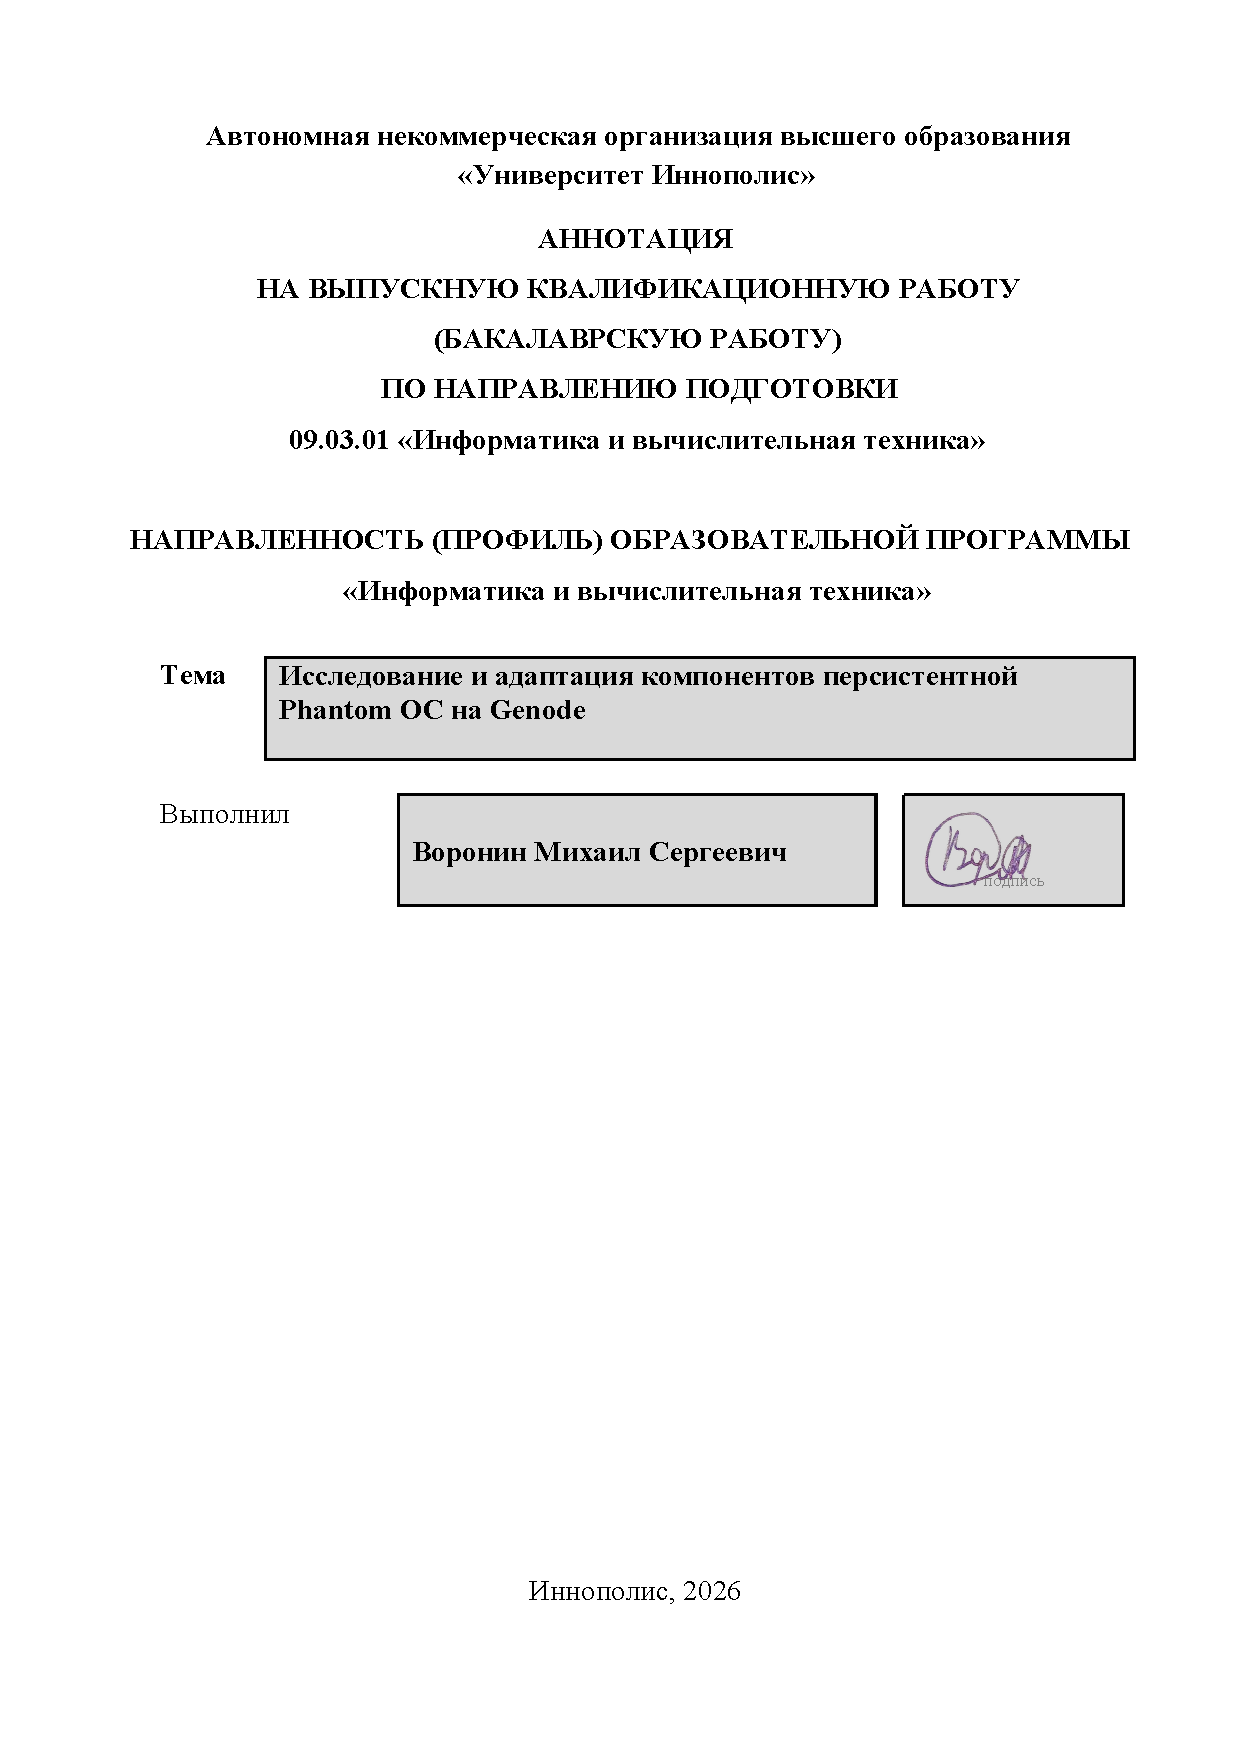
\includepdf[offset=2.5cm -2.2cm, pages=-, pagecommand={\thispagestyle{empty}}]{title_signed.pdf}
\setcounter{page}{2}
\tableofcontents
% \setcounter{page}{4}
% set manually the number, from which Глава 1 starts!
% Why do we put 4 in this case?
% Title page - page 1
% Оглавление - page 2
% Аннотация - page 3
% Глава 1 - page 4
% In your annotation the counter number can be different, please count carefully and insert the corresponding number.

% \chapter{Введение}

Актуальность работы обусловлена тем, что современные операционные системы используют модель управления памятю, сложившуюся с появлением UNIX. Она требует от программиста явного сохранения данных на диск, что увеличивает объём кода и приводит к потерям при сбоях~\cite{PLA}. Концепция персистентности устраняет эти недостатки, однако её практические реализации на современном оборудовании по-прежнему остаются предметом исследований~\cite{Revisited,Aurora}.

Работа выполнена в контексте проекта по портированию Phantom~OS на Genode. Phantom~OS реализует ортогональную персистентность внутри Phantom Virtual Machine~(PVM), периодически сохраняя её состояние на диск ~\cite{Phantom_docs}. Снапшоты хранятся в открытом виде, что создаёт угрозу конфиденциальности: в момент снимка в памяти могут быть секретные данные в открытом виде~\cite{SNIA_PM_Security,VM_Security}. \textbf{Цель работы}~--- обеспечить конфиденциальность снапшотов в состоянии покоя. Для этого адаптирован компонент, который реализует шифрование на блочном уровне, используя библиотеку Tresor, проведена верификация защиты и оценено влияние на производительность.

% \chapter{Краткое описание основной части работы}

Основная часть состоит из шести глав: введение, обзор литературы, методология, реализация, оценка и обсуждение, заключение.

Глава~1 формулирует проблему: снапшоты содержат полный слепок памяти PVM, включая конфиденциальные данные, и хранятся без шифрования. Описаны предпосылки появления ортогональной персистентности, архитектура PhantomOS~\cite{Phantom_docs} и Genode~\cite{Genode_Foundations}, поставлены цели и задачи.

Глава~2 представляет обзор литературы по четырём направлениям. Рассматривается концепция ортогональной персистентности~\cite{PLA,Revisited,KOS,Aurora} и её реализация в PhantomOS. Описана история порта PhantomOS на Genode~\cite{Antonov_Anton} и механизм Snapper~2.0~\cite{FOSDEM_Snapper,FOSDEM_Snapper_paper}. Приводится классификация методов шифрования данных в состоянии покоя~\cite{NIST_SP800111,CryptoFS} и обосновывается выбор блочного шифрования с использованием библиотеки Tresor.

Глава~3 описывает методологию. На основе модели сценариев использования (граф состояний от включения до выключения) выбраны безопасные сценарии с аутентификацией через USB-накопитель с ключом. Сформулированы четыре требования: обязательная авторизация, хранение ключей на USB, шифрование снапшотов, гарантия записи только зашифрованных данных. Определён план реализации на базе существующего компонента \texttt{file\_vault}.

Глава~4 описывает реализацию компонента \texttt{se\_vault}. Графический интерфейс удалён, аутентификация перенесена на USB, файловая система сменена с ext2 на ext4~(\texttt{lwext4}), добавлена поддержка fsck, блочная сессия передаётся в Tresor напрямую, все блоки унифицированы до~4~КБ. В \texttt{lwext4} исправлена функция \texttt{ftruncate} и добавлена передача \texttt{sync} на нижние уровни VFS. В компонентах isomem, snapper и vfs реализована корректная цепочка завершения. Тестирование в QEMU подтвердило корректность шифрования и восстановления из снапшота. Нагрузочные тесты выявили снижение производительности в~$\approx$25~раз (первый снапшот: $\approx$2~с без шифрования и $\approx$51~с с шифрованием) из-за однопоточной реализации Tresor; инициализация ускорилась с~$\approx$20~мин до~$\approx$1~мин.

Глава~5 содержит оценку результатов. Проведён сравнительный анализ \texttt{file\_vault} и \texttt{se\_vault}; рассмотрены ограничения, связанные с непроизводственным статусом Tresor и тестированием в виртуальной среде; обсуждаются пути решения проблемы производительности.

% \chapter{Заключение}

Компонент \texttt{se\_vault} адаптирован для шифрования снапшотов PhantomOS в рамках её порта на Genode. Система решает задачу обеспечения конфиденциальности снапшотов в состоянии покоя и для остальных компонентов порта интегрируется прозрачно.

Поставленные задачи выполнены: адаптирован компонент блочного шифрования, верифицирована недоступность содержимого снапшота без ключа, оценено влияние шифрования на производительность. Цель достигнута частично: защита снапшотов реализована, однако производительность значительно снизилась из-за ограничений библиотеки Tresor.

Ограничения текущей работы связаны с эксперементальной реализацией Tresor и тестированием только в виртуальной среде. Дальнейшие направления исследований: оптимизация Tresor, распространение шифрования на блочное устройство isomem, возможное объединение Snapper и Tresor~\cite{FOSDEM_Snapper_paper}.


\section{Введение}

Актуальность работы обусловлена тем, что современные операционные системы используют модель управления памятю, сложившуюся с появлением UNIX. Она требует от программиста явного сохранения данных на диск, что увеличивает объём кода и приводит к потерям при сбоях~\cite{PLA}. Концепция персистентности устраняет эти недостатки, однако её практические реализации на современном оборудовании по-прежнему остаются предметом исследований~\cite{Revisited,Aurora}.

Работа выполнена в контексте проекта по портированию Phantom~OS на Genode. Phantom~OS реализует ортогональную персистентность внутри Phantom Virtual Machine~(PVM), периодически сохраняя её состояние на диск ~\cite{Phantom_docs}. Снапшоты хранятся в открытом виде, что создаёт угрозу конфиденциальности: в момент снимка в памяти могут быть секретные данные в открытом виде~\cite{SNIA_PM_Security,VM_Security}. \textbf{Цель работы}~--- обеспечить конфиденциальность снапшотов в состоянии покоя. Для этого адаптирован компонент, который реализует шифрование на блочном уровне, используя библиотеку Tresor, проведена верификация защиты и оценено влияние на производительность.

\section{Краткое описание основной части работы}

Основная часть состоит из пяти глав: введение, обзор литературы, методология, реализация, оценка и обсуждение.

Глава~1 формулирует проблему: снапшоты содержат полное состояние памяти PVM, включая конфиденциальные данные, и хранятся без шифрования. Описаны предпосылки появления ортогональной персистентности, архитектура PhantomOS~\cite{Phantom_docs} и Genode~\cite{Genode_Foundations}, поставлены цели и задачи.

Глава~2 представляет обзор литературы по четырём направлениям. Рассматривается концепция ортогональной персистентности~\cite{PLA,Revisited,KOS,Aurora} и её реализация в PhantomOS. Описываются текущее состояние порта PhantomOS на Genode~\cite{Antonov_Anton} и Snapper~2.0~\cite{FOSDEM_Snapper,FOSDEM_Snapper_paper}. Приводится классификация методов шифрования данных в состоянии покоя~\cite{NIST_SP800111,CryptoFS} и обосновывается выбор блочного шифрования с использованием библиотеки Tresor.

Глава~3 описывает методологию. На основе модели сценариев использования (граф, описывающий полный цикл работы компьютера) выбраны безопасные сценарии с аутентификацией по фактору наличия USB-накопителя с ключом. Сформулированы четыре требования: обязательная авторизация, хранение ключей на USB, шифрование снапшотов, гарантия хранения только зашифрованных данных. Определён план реализации на базе существующего компонента \texttt{file\_vault}.

Глава~4 описывает процесс адаптации компонента \texttt{se\_vault} для хранения снапшотов. Графический интерфейс удалён, парольная аутентификация заменена на аутентификацию по USB, файловая система заменена с ext2 на ext4~(\texttt{lwext4}), вместо VFS-плагина \texttt{rump} внедрен \texttt{lwext4} добавлена поддержка fsck, блочная сессия передаётся в Tresor напрямую, все блоки унифицированы до~4~КБ. В \texttt{lwext4} исправлена функция \texttt{ftruncate} и добавлена передача \texttt{sync} на нижние уровни VFS. В компонентах isomem, snapper и vfs реализована корректная цепочка завершения. Тестирование в QEMU подтвердило корректность шифрования и возможность восстановления из снапшота. Нагрузочные тесты выявили снижение производительности в~$\approx$25~раз (первый снапшот: $\approx$2~с без шифрования и $\approx$51~с с шифрованием) из-за низкого уровня оптимизации Tresor; инициализация адаптированного компонента сократилась с~$\approx$20~мин до~$\approx$1~мин в сравнении с оригинальным.

Глава~5 содержит оценку результатов. Проведён сравнительный анализ \texttt{file\_vault} и \texttt{se\_vault} (адаптированная версия); рассмотрены ограничения, связанные с эксперементальной реализацией Tresor и тестированием в виртуальной среде; обсуждаются пути решения проблемы производительности.

\section{Заключение}

Компонент \texttt{se\_vault} адаптирован для шифрования снапшотов PhantomOS в рамках её порта на Genode. Система решает задачу обеспечения конфиденциальности снапшотов в состоянии покоя и для остальных компонентов порта интегрируется прозрачно.

Поставленные задачи выполнены: адаптирован компонент блочного шифрования, верифицирована недоступность содержимого снапшота без ключа, оценено влияние шифрования на производительность. Цель достигнута частично: защита снапшотов реализована, однако производительность значительно снизилась из-за ограничений библиотеки Tresor.

Ограничения текущей работы связаны с эксперементальной реализацией Tresor и тестированием только в виртуальной среде. Дальнейшие направления исследований: оптимизация Tresor, распространение шифрования на блочное устройство isomem, возможное объединение Snapper и Tresor~\cite{FOSDEM_Snapper_paper}.


\printbibliography[heading=bibintoc,title={Список использованной литературы}]
\end{document}

